% The von Neumann universe V drawn as a triangle built in layers
% V_0 = ∅ ⊆ V_1 ⊆ V_2 ⊆ ... indexed by the ordinals On.
% Source: book/tex/set-theory/ordinal.tex (§ The von Neumann universe).
\documentclass[border=2mm]{standalone}
\usepackage{tikz}
\usepackage{amssymb}
\begin{document}
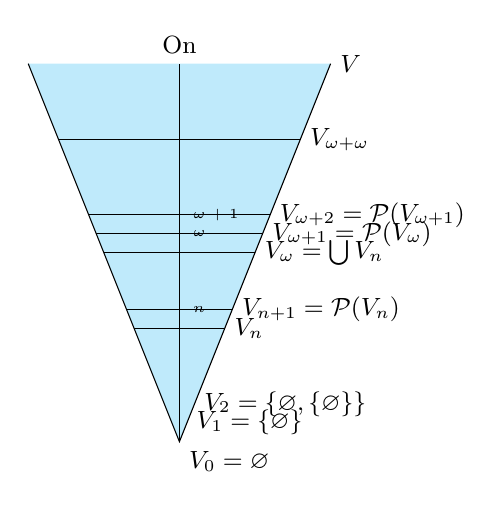
\begin{tikzpicture}[scale=0.16, every node/.style={font=\small}]
  \fill[cyan!25] (0,0) -- (12,30) -- (-12,30) -- cycle;
  \draw (12,30) -- (0,0) -- (-12,30);
  \draw (0,0) -- (0,30);
  \node[above] at (0,30) {$\mathrm{On}$};
  \node[right] at (12,30) {$V$};
  % low levels: labels only (they crowd the apex)
  \node[below right] at (0,0) {$V_0 = \varnothing$};
  \node[right] at (0.6,1.5) {$V_1 = \{\varnothing\}$};
  \node[right] at (1.2,3) {$V_2 = \{\varnothing, \{\varnothing\}\}$};
  % drawn levels
  \draw (-3.6,9) -- (3.6,9) node[right] {$V_n$};
  \draw (-4.2,10.5) -- (4.2,10.5) node[right] {$V_{n+1} = \mathcal{P}(V_n)$};
  \draw (-6,15) -- (6,15) node[right] {$V_\omega = \bigcup V_n$};
  \draw (-6.6,16.5) -- (6.6,16.5) node[right] {$V_{\omega+1} = \mathcal{P}(V_\omega)$};
  \draw (-7.2,18) -- (7.2,18) node[right] {$V_{\omega+2} = \mathcal{P}(V_{\omega+1})$};
  \draw (-9.6,24) -- (9.6,24) node[right] {$V_{\omega+\omega}$};
  \node[right] at (0.3,10.5) {\tiny $n$};
  \node[right] at (0.3,16.5) {\tiny $\omega$};
  \node[right] at (0.3,18) {\tiny $\omega+1$};
\end{tikzpicture}
\end{document}
